% Source: AESP_466_ClassWork/Supplements/Notes/latex/5.3.4/5.3.4.tex

\documentclass[border=4pt]{standalone}
\usepackage{amsmath,amssymb,amsthm}
\usepackage{graphicx}
\usepackage{tikz}
\usepackage{xcolor}
\usetikzlibrary{arrows.meta,calc,positioning,decorations.markings,patterns,shapes.geometric,angles,quotes}

\definecolor{Garnet}{HTML}{73000A}
\definecolor{USC_Rose}{HTML}{CC2E40}
\definecolor{USC_Blue}{HTML}{466A9F}
\definecolor{USC_Slate}{HTML}{1F414D}
\definecolor{USC_Olive}{HTML}{65780B}
\definecolor{USC_Lime}{HTML}{CED318}
\definecolor{USC_Gold}{HTML}{A49137}
\definecolor{USC_Black90}{HTML}{565556}
\definecolor{USC_Black10}{HTML}{ECECEC}

\newcommand{\vect}[1]{\mathbf{#1}}
\newcommand{\mat}[1]{\mathbf{#1}}
\newcommand{\uvec}[1]{\hat{\mathbf{#1}}}
\newcommand{\transpose}{^{\mkern-1.5mu\mathsf{T}}}
\newcommand{\inv}{^{-1}}
\newcommand{\deriv}[2]{\frac{d #1}{d #2}}
\newcommand{\pderiv}[2]{\frac{\partial #1}{\partial #2}}

\begin{document}
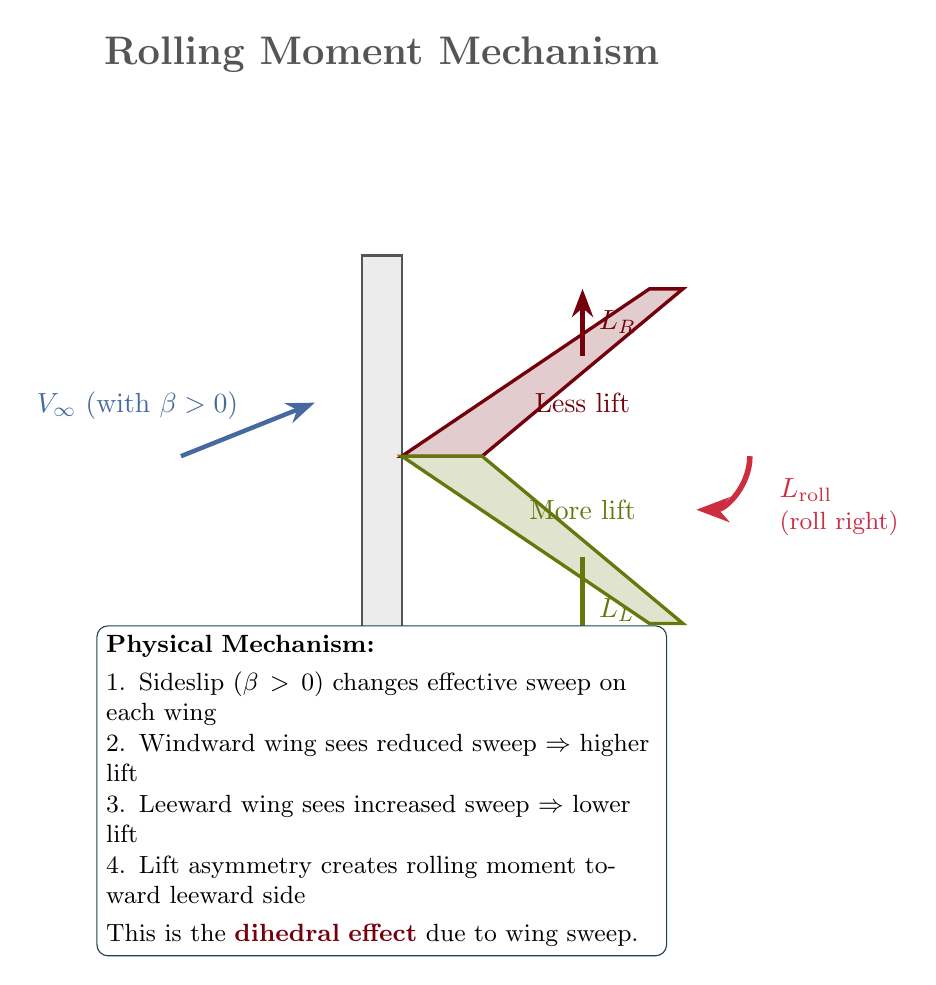
\begin{tikzpicture}[>=Stealth, scale=0.85]
    % Title
    \node[font=\Large\bfseries, USC_Black90] at (0,6) {Rolling Moment Mechanism};

    % Aircraft top view (simplified)
    % Fuselage
    \draw[thick, USC_Black90, fill=USC_Black10] (-0.3,-3) rectangle (0.3,3);

    % Right wing (more lift due to reduced effective sweep)
    \draw[very thick, Garnet, fill=Garnet!20] (0.3,0) -- (4,2.5) -- (4.5,2.5) -- (1.5,0) -- cycle;
    \node[Garnet] at (3,0.8) {Less lift};

    % Left wing (less lift due to increased effective sweep)
    \draw[very thick, USC_Olive, fill=USC_Olive!20] (0.3,0) -- (4,-2.5) -- (4.5,-2.5) -- (1.5,0) -- cycle;
    \node[USC_Olive] at (3,-0.8) {More lift};

    % Lift arrows
    \draw[->, ultra thick, Garnet] (3,1.5) -- (3,2.5);
    \node[Garnet, right] at (3.1,2) {$L_R$};

    \draw[->, ultra thick, USC_Olive] (3,-1.5) -- (3,-3);
    \node[USC_Olive, right] at (3.1,-2.3) {$L_L$};

    % Sideslip velocity
    \draw[->, ultra thick, USC_Blue] (-3,0) -- (-1,0.8);
    \node[USC_Blue, above left] at (-2,0.4) {$V_\infty$ (with $\beta > 0$)};

    % Rolling moment arrow
    \draw[->, ultra thick, USC_Rose, line width=2pt] (5.5,0) arc (0:-90:0.8);
    \node[USC_Rose, right] at (5.8,-0.5) {$L_{\text{roll}}$};
    \node[USC_Rose, right, font=\small] at (5.8,-1) {(roll right)};

    % Explanation box
    \node[draw=USC_Slate, fill=white, rounded corners, align=left, font=\small, text width=7cm] at (0,-5) {
        \textbf{Physical Mechanism:}\\[0.3em]
        1. Sideslip ($\beta > 0$) changes effective sweep on each wing\\
        2. Windward wing sees reduced sweep $\Rightarrow$ higher lift\\
        3. Leeward wing sees increased sweep $\Rightarrow$ lower lift\\
        4. Lift asymmetry creates rolling moment toward leeward side\\[0.3em]
        This is the \textcolor{Garnet}{\textbf{dihedral effect}} due to wing sweep.
    };

\end{tikzpicture}
\end{document}
